\documentclass[a4paper]{article}
\usepackage[T1]{fontenc}
\usepackage[utf8]{inputenc}
\usepackage[english]{babel}
\usepackage{frontespizio}
\usepackage{graphicx}
\usepackage{subfig}
\usepackage{listings}
\usepackage{scrextend}
\usepackage[margin=1.2in]{geometry}
\usepackage[font=small,labelfont=bf]{caption}
\usepackage{url}

\begin{document}
\selectlanguage{english}
\baselineskip 13pt
	
% ---- FRONTESPIZIO ----- 
\begin{frontespizio} 
 \Preambolo{\renewcommand{\frontpretitlefont}{\fontsize{15}{12}\scshape}}
\Istituzione {University of Pisa}
\Divisione {Scuola di Ingegneria}
\Corso [Laurea]{Artificial Intelligence and Data Engineering}
\Annoaccademico {2019--2020}
\Titolo { \vspace {35mm}Documentation of the\\"STAD" Application}
\Filigrana [height=4cm,before=0.28,after=1]{./images/stemma_unipi.png}
\Rientro {1cm}
\Candidato {Alice Nannini}
\Candidato {Marco Parola}
\Relatore {Prof. Francesco Marcelloni}
\Relatore {Prof. Pietro Ducange}
 \Punteggiatura {}
\end{frontespizio}


% ----- INDICE -----
\tableofcontents\thispagestyle{empty}
\clearpage


\section{Introduction}\pagenumbering{arabic}
The goal of this application is to prevent and detect situations potentially dangerous, caused by huge amounts of rain, scraping twitter and analyzing each tweet, in order to discover some tweets containing information related to these critical situations.\\
We analyze the data and develop the application using Python and Sklearn library.

\section{The Data}
\subsection{Retrieve the data}
The data, on which this application works, are tweets. In order to collect enought tweets, we scraped twitter, using \textbf{twint}.\\
Twint is an advanced opensource Twitter scraping tool, written in Python, thanks to which it's very easy to collect data, according to some criteria, and store them in csv files.
For more information about \textit{twintproject} visit the Github repository: \url{https://github.com/twintproject}.
\begin{verbatim}
   twint -s <WORDS> -o tweetPioggia.csv --csv

   <WORDS> : 'pioggia', 'piove', 'allerta', 'meteo', 'alluvione', 'maltempo'
\end{verbatim}
Examples:
\begin{itemize}
\item "Ora piove a dirotto per la gioia di yuki che non può andare al parco"
\item "Ma dai, ma piove sul bagnato! Povera Antonella!!!!! \#GFVIP"
\end{itemize}
Moreover we added to the dataset some posts randomly downloaded, not related to any weather phenomenons (without specifying any keywords).

\subsection{Prepare the dataset}
After collectioning the tweets (902), we assigned each of them to a class, in order to prepare the dataset, thanks to which we can build some classifiers.\\
We decided to map the tweets in 3 classes:
\begin{itemize}
\item 0 -> the tweet is not related to a weather condition (376)
\item 1 -> the tweet is about rain or some weather condition not dangerous (224)
\item 2 -> the tweet is about some dangerous situation caused by the rain (302)
\end{itemize}

\section{Preprocessing}
In this phase, we first extract from the \textit{csv} file, created by \emph{twint}, just the tweets' texts, discarding all the meta-information associated with them (id, user, etc.).\\
Then we delete some tweets, in order to manage only the italian tweets. The deleting is made using the \textit{guess\_language} package.\\
Finally, we clean the text of each tweet removing eventual URLs: to do so, we use a Regular Expression filter.

\section{Supervised learning stage}
%\section{Text Elaboration}
After the preprocessing phase, we follow the standard steps to build our classification model, managing the tweets' texts:
\begin{itemize}
\item tokenization, stop-word filtering and stemming
\item stem filtering by relevant stems, selected by the tf-idf computation
\item classification and evaluation
\end{itemize}

\subsection{Tokenization, stop-word filtering and stemming}
After stratified splitting the dataset in tranining and test set, we tokenize each tweet and we apply an italian stemming filter, in order to find more general words.
\begin{verbatim}
   italian_stemmer = SnowballStemmer('italian')
   class StemmedCountVectorizer(CountVectorizer):
      def build_analyzer(self):
         analyzer = super(StemmedCountVectorizer, self).build_analyzer()
         return lambda doc: ([italian_stemmer.stem(w) for w in analyzer(doc)])
\end{verbatim}

\subsection{Stem filtering by relevant stems}
All the stems are united in one vector and are weighted using the IDF index (Inverse Document Frequency).\\
Then, each training tweet is represented as a vector of features, dimension equal to the number of stems, and the i-th feature is calculated as the frequency of the i-th stem in the tweet per the weight of that stem.\\
Finally each stem is evaluated by the Information Gain (IG) value between the corresponding feature and the possible class labels:
\begin{verbatim}
   IG(C, Sq) = H(C) - H(C|Sq)
\end{verbatim}
where $Sq$ is the feature corresponding to the stem $s_q$, $H(C)$ is the entropy of $C$, and $H(C|Sq)$ is the entropy of $C$ after the observation of the feature $Sq$.\\
Then, the stems are ranked in descending order and $F$ stems, with $F \leq Q$, are selected among these.
\begin{verbatim}
   tfidf_transformer = TfidfTransformer(smooth_idf=True,use_idf=True)
   X_train_tfidf = tfidf_transformer.fit_transform(X_train_counts)
\end{verbatim}

\subsection{Classification and evaluation}
After the tfidf\_transformer fitting phase, we use it to transform the test set and we build and test different classifiers and compute different metrics to compare them (accurancy, f-score, confusion-matrix):
\begin{verbatim}
Multinomial NB:
accuracy : 0.7822878228782287
f_score : 0.7217817028974173


Decision Tree:
accuracy : 0.8191881918819188
f_score : 0.8005383709471964

SVM:
accuracy : 0.7970479704797048
f_score : 0.7676179382644147

k-NN (k=5):
accuracy : 0.5276752767527675
f_score : 0.38181323539413725

Adaboost:
accuracy : 0.7712177121771218
f_score : 0.7538220246286299

Random Forest:
accuracy : 0.8376383763837638
f_score : 0.8169722687103137
\end{verbatim}

\begin{figure}[b]
\centering
\subfloat[][\emph{Random Forest}]
{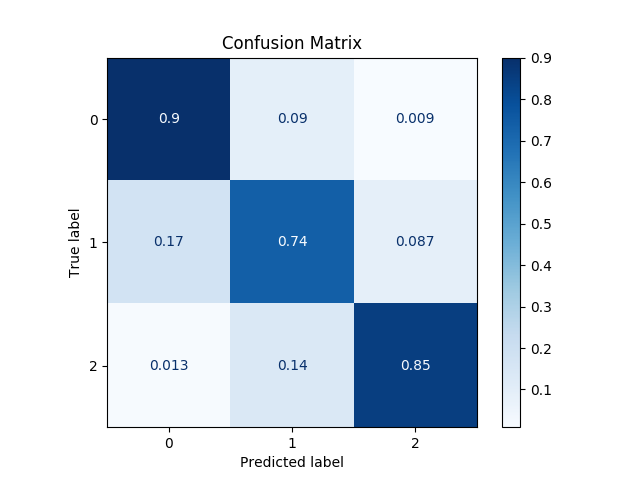
\includegraphics[width=0.45\textwidth]{images/randomForest}}
\subfloat[][\emph{Multinomial Naive-Bayes}]
{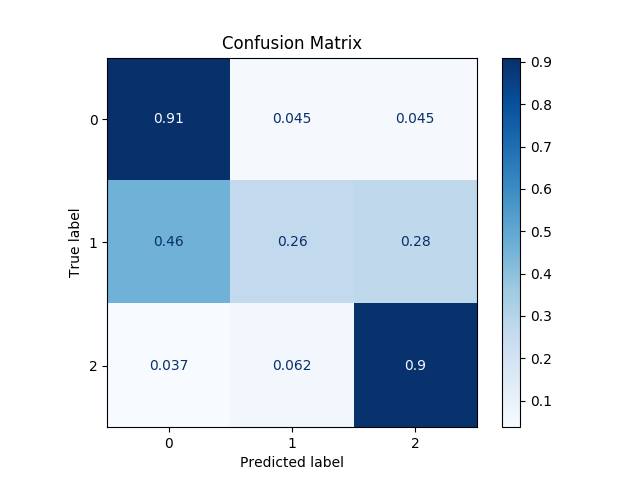
\includegraphics[width=0.45\textwidth]{images/gaussian}} \\
\subfloat[][\emph{SVM}]
{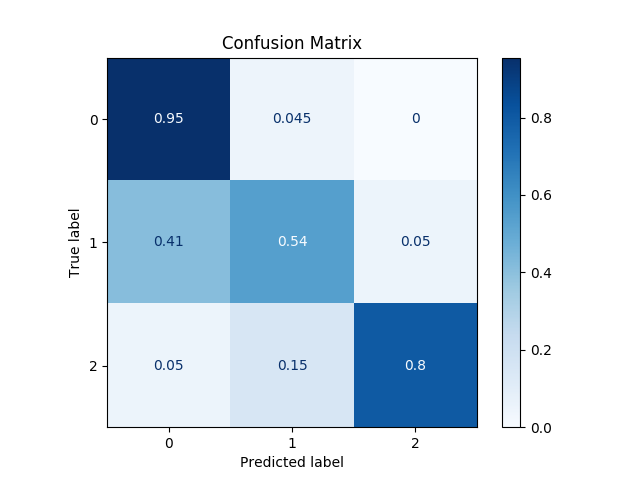
\includegraphics[width=0.45\textwidth]{images/svc}}
\subfloat[][\emph{Decision Tree}]
{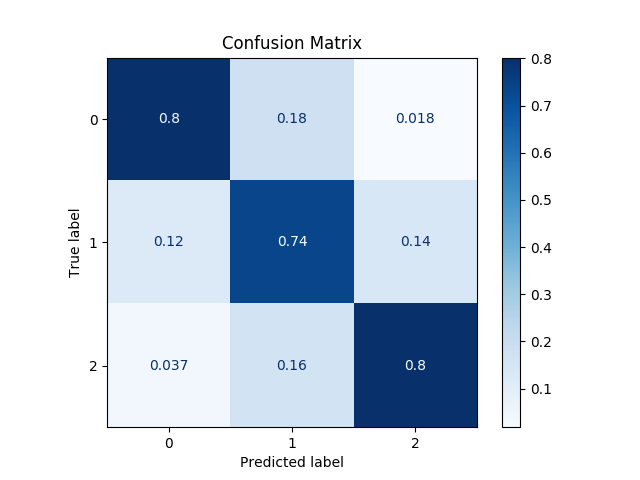
\includegraphics[width=0.45\textwidth]{images/decisionTree}} \\
\subfloat[][\emph{k Nearest Neighbors (k = 5)}]
{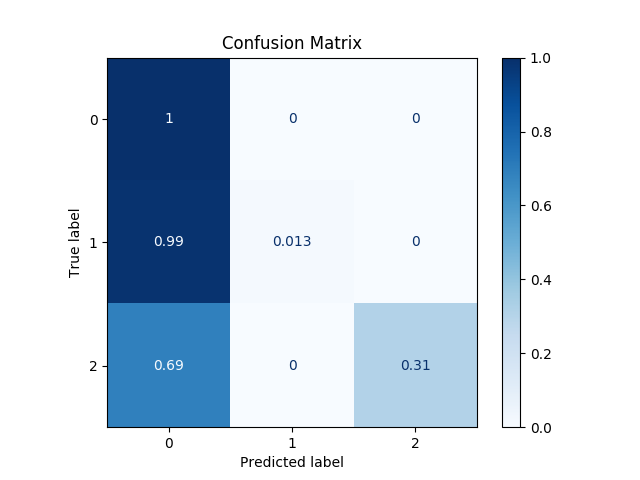
\includegraphics[width=0.45\textwidth]{images/knn}}
\subfloat[][\emph{Adaboost}]
{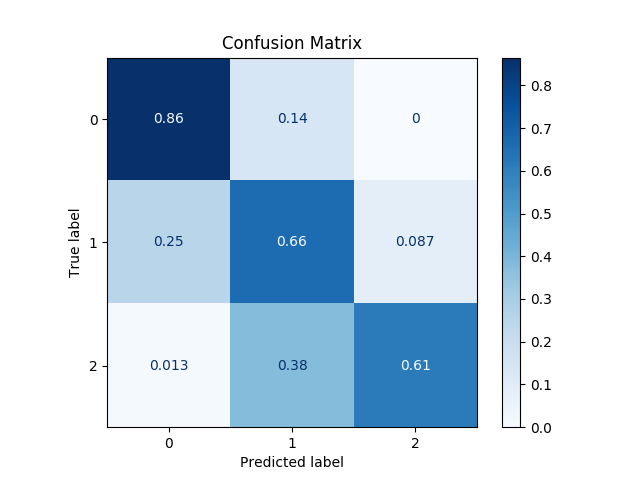
\includegraphics[width=0.45\textwidth]{images/adaBoost}} \\
\caption{}
\label{fig:confusion_matrices}
\end{figure}

\subsection{Cross-validation}
We try to evaluate all the previous phases of elaboration and supervised learning, based on our dataset, with the method of cross-validation. Using 10 folds, these are our results for each classifier involved:
\begin{verbatim}
Accuracy MultinomialNB : 0.75 (+/- 0.10)
Accuracy Decision Tree : 0.77 (+/- 0.22)
Accuracy SVM : 0.80 (+/- 0.16)
Accuracy k-NN : 0.68 (+/- 0.17)
Accuracy Adaboost : 0.72 (+/- 0.22)
Accuracy Random Forest : 0.81 (+/- 0.21)
\end{verbatim}

Given the results obtained both in single evaluation and in cross-validation, we conclude that the SVM classifier is the best for our application. Indeed, it has the higher accuracy, second just to the Random Forest's one. Moreover, this last algorithm has larger confidence intervals ($\pm 2std$) than the SVM, that is to prefer. 

\section{Experimental results}
We select some significant events of strong weather conditions, involving rain and flooding, happened in Italy during the past years. We collect the tweets posted on the social network during the hours of each event and then we pass these data to our new constructed model. The selected events are:
\begin{itemize}
\item flood in Casteldaccia, province of Palermo, 2018-11-03
\begin{verbatim}
twint -g="38.1405227,13.2870764,50km" --since 2018-11-02 --until 2018-11-05 
-o palermo2018.csv --csv
\end{verbatim}
\item flood in Piemonte, 2016-11-21/25
\begin{verbatim}
twint -g="45.0704900,7.6868200,50km" --since 2016-11-23 --until 2016-11-26 
-o piemonte2016.csv --csv
\end{verbatim}
\end{itemize}
Then, we select also a day with no significant weather conditions, and we apply the model on the data retrieved also from that day:
\begin{verbatim}
twint --near Pisa --since 2020-02-21 --until 2020-02-22 -o pisa2020.csv --csv
\end{verbatim}


\end{document}